The assembly of the structure involves the integration of the array of all actuators, the platform on which they are mounted, and the electronics responsible for controlling the linear actuators. The components of the platform are shown in Figure \ref{fig:platform-assembly}, and the corresponding parts list is detailed in Table \ref{tab:platform-assembly}. The structure features a hexagonal shape but includes only three lateral structural supports, made of acrylic, as well as the upper and lower bases, which are also made of acrylic. These components are connected using 3D-printed L-shaped joints. There is a hollow space beneath the actuators to provide clearance for the rods, approximately 25 centimeters in length.


\begin{figure}
    \centering
    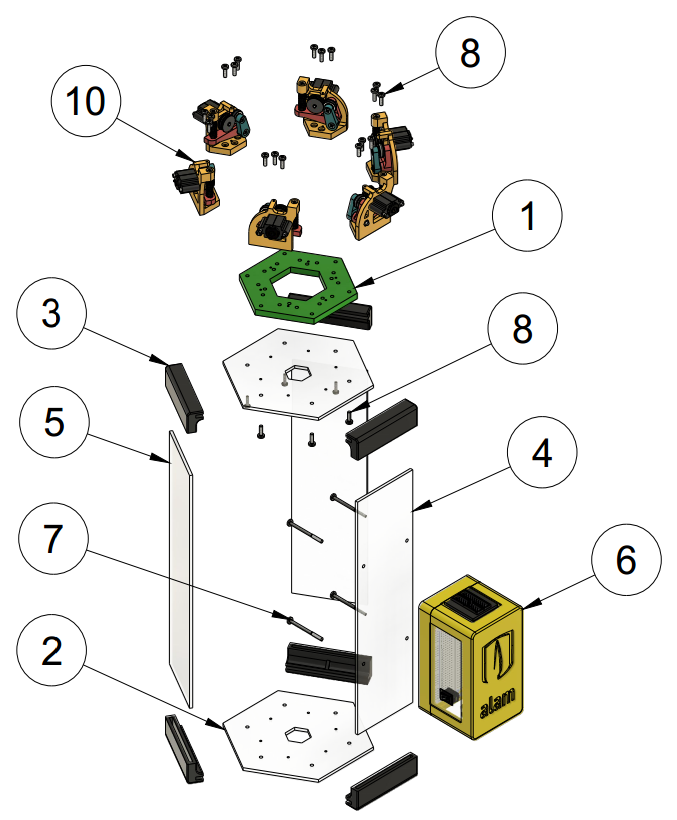
\includegraphics[width=0.7\textwidth]{platform-assembly}
    \caption{Platform assembly exploded-view}
    \label{fig:platform-assembly}
\end{figure}

\begin{table}[]
    \centering
    \caption{Platform assembly parts list}
    \label{tab:platform-assembly}
    \begin{tabular}{llll}
    \toprule
    Item & Qty & Part Name / Description & Source \\
    \midrule
    1 & 1 & Actuators Base & 3D Printed \\
    2 & 2 & Support Base & Acrylic Laser Cut \\
    3 & 6 & Support Union & Acrylic Laser Cut \\
    4 & 1 & Support Front & Acrylic Laser Cut \\
    5 & 2 & Support Lateral & Acrylic Laser Cut \\
    6 & 1 & Electronics Assembly & \\
    7 & 4 & Binding Head Screw JIS B 1111 - M3x40 & Commercial \\
    8 & 24 & Binding Head Screw JIS B 1111 - M3x10 & Commercial \\
    9 & 6 & Actuator Assembly & \\
    \bottomrule
    \end{tabular}
\end{table}


\section{Electronics Case}

The electronics case houses all the electronic components necessary to control the motors. It is an independent module from the platform structure, making it easy to remove and replace, and it is positioned beside the platform for easy access. The case contains the MCU (Microcontroller Unit), the breadboard on which the motor drivers and various connections are made, as well as the input and output peripherals of the module, which can be seen in Figure \ref{fig:electronics-assembly} and are listed in Table \ref{tab:electronics-assembly}. The case consists of two main parts, one containing the MCU and the other housing the breadboard, both of which are 3D-printed. The peripherals are mounted on the walls, which are made of laser-cut acrylic sheets.

\begin{figure}[H]
    \centering
    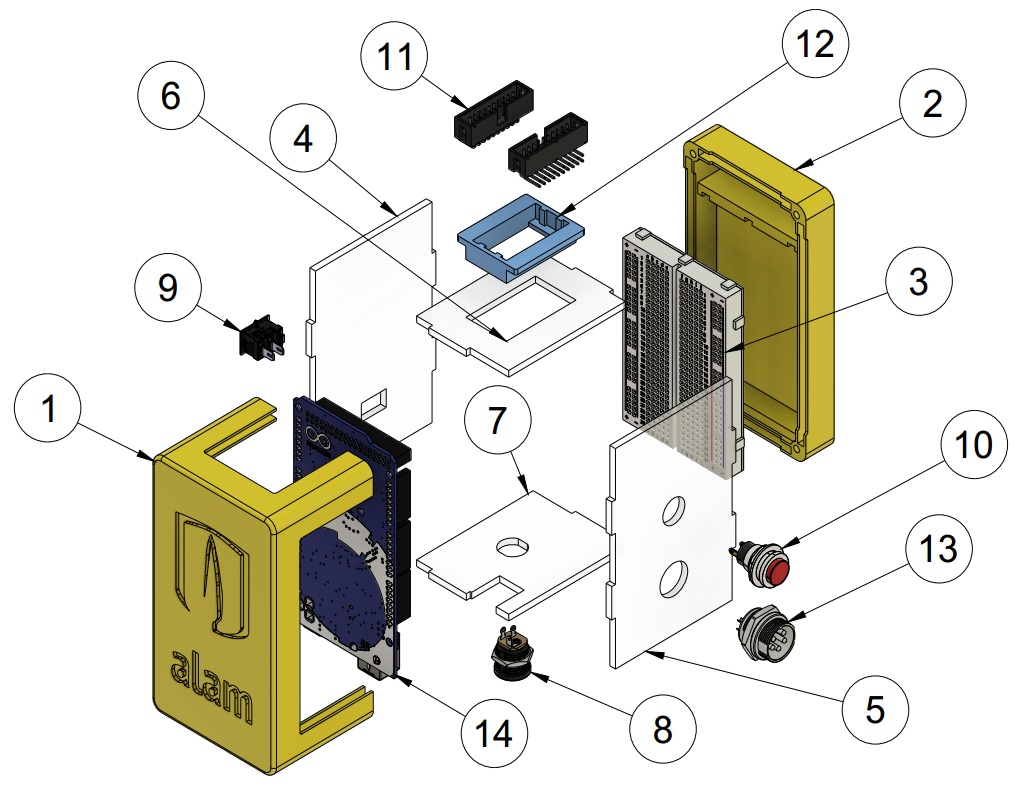
\includegraphics[width=0.8\textwidth]{electronics-assembly}
    \caption{Electronics assembly exploded-view}
    \label{fig:electronics-assembly}
\end{figure}

\begin{table}[h]
    \centering
    \caption{Electronics assembly parts list}
    \label{tab:electronics-assembly}
    \begin{tabular}{llll}
    \toprule
    Item & Qty & Part Name / Description & Source \\
    \midrule
    1 & 1 & Arduino Case & 3D Printed \\
    2 & 1 & Breadboard Base & 3D Printed \\
    3 & 1 & Half-Size Breadboard & Commercial \\
    4 & 1 & Left Wall & Acrylic Laser Cut \\
    5 & 1 & Right Wall & Acrylic Laser Cut \\
    6 & 1 & Top Wall & Acrylic Laser Cut \\
    7 & 1 & Bottom Wall & Acrylic Laser Cut \\
    8 & 1 & DC Power Input Jack - DS-223B & Commercial \\
    9 & 1 & Power Switch - KCD1-11-2P & Commercial \\
    10 & 1 & Red Push Button - DS 212 & Commercial \\
    11 & 2 & IDC 3020-20-0200-00 - 20P 2.54MM & Commercial \\
    12 & 1 & IDC Support & 3D Printed \\
    13 & 1 & MX M12 5-Pin Male MIC Connector Plug & Commercial \\
    14 & 1 & Arduino MEGA 2650 & Commercial \\
    \bottomrule
    \end{tabular}
\end{table}

Figure \ref{fig:electronics-ports} shows the ports and connections of the case: on the bottom, there is the serial port input for programming the MCU and sending commands, and the power plug; on the right side, there is an emergency button to stop the robot, and a 5-pin connector input for connecting a joystick; on the left side, there is the power button; and on the top, there are a pair of 20-pin IDC inputs for connecting the unit to the motors.

\begin{figure}
    \centering
    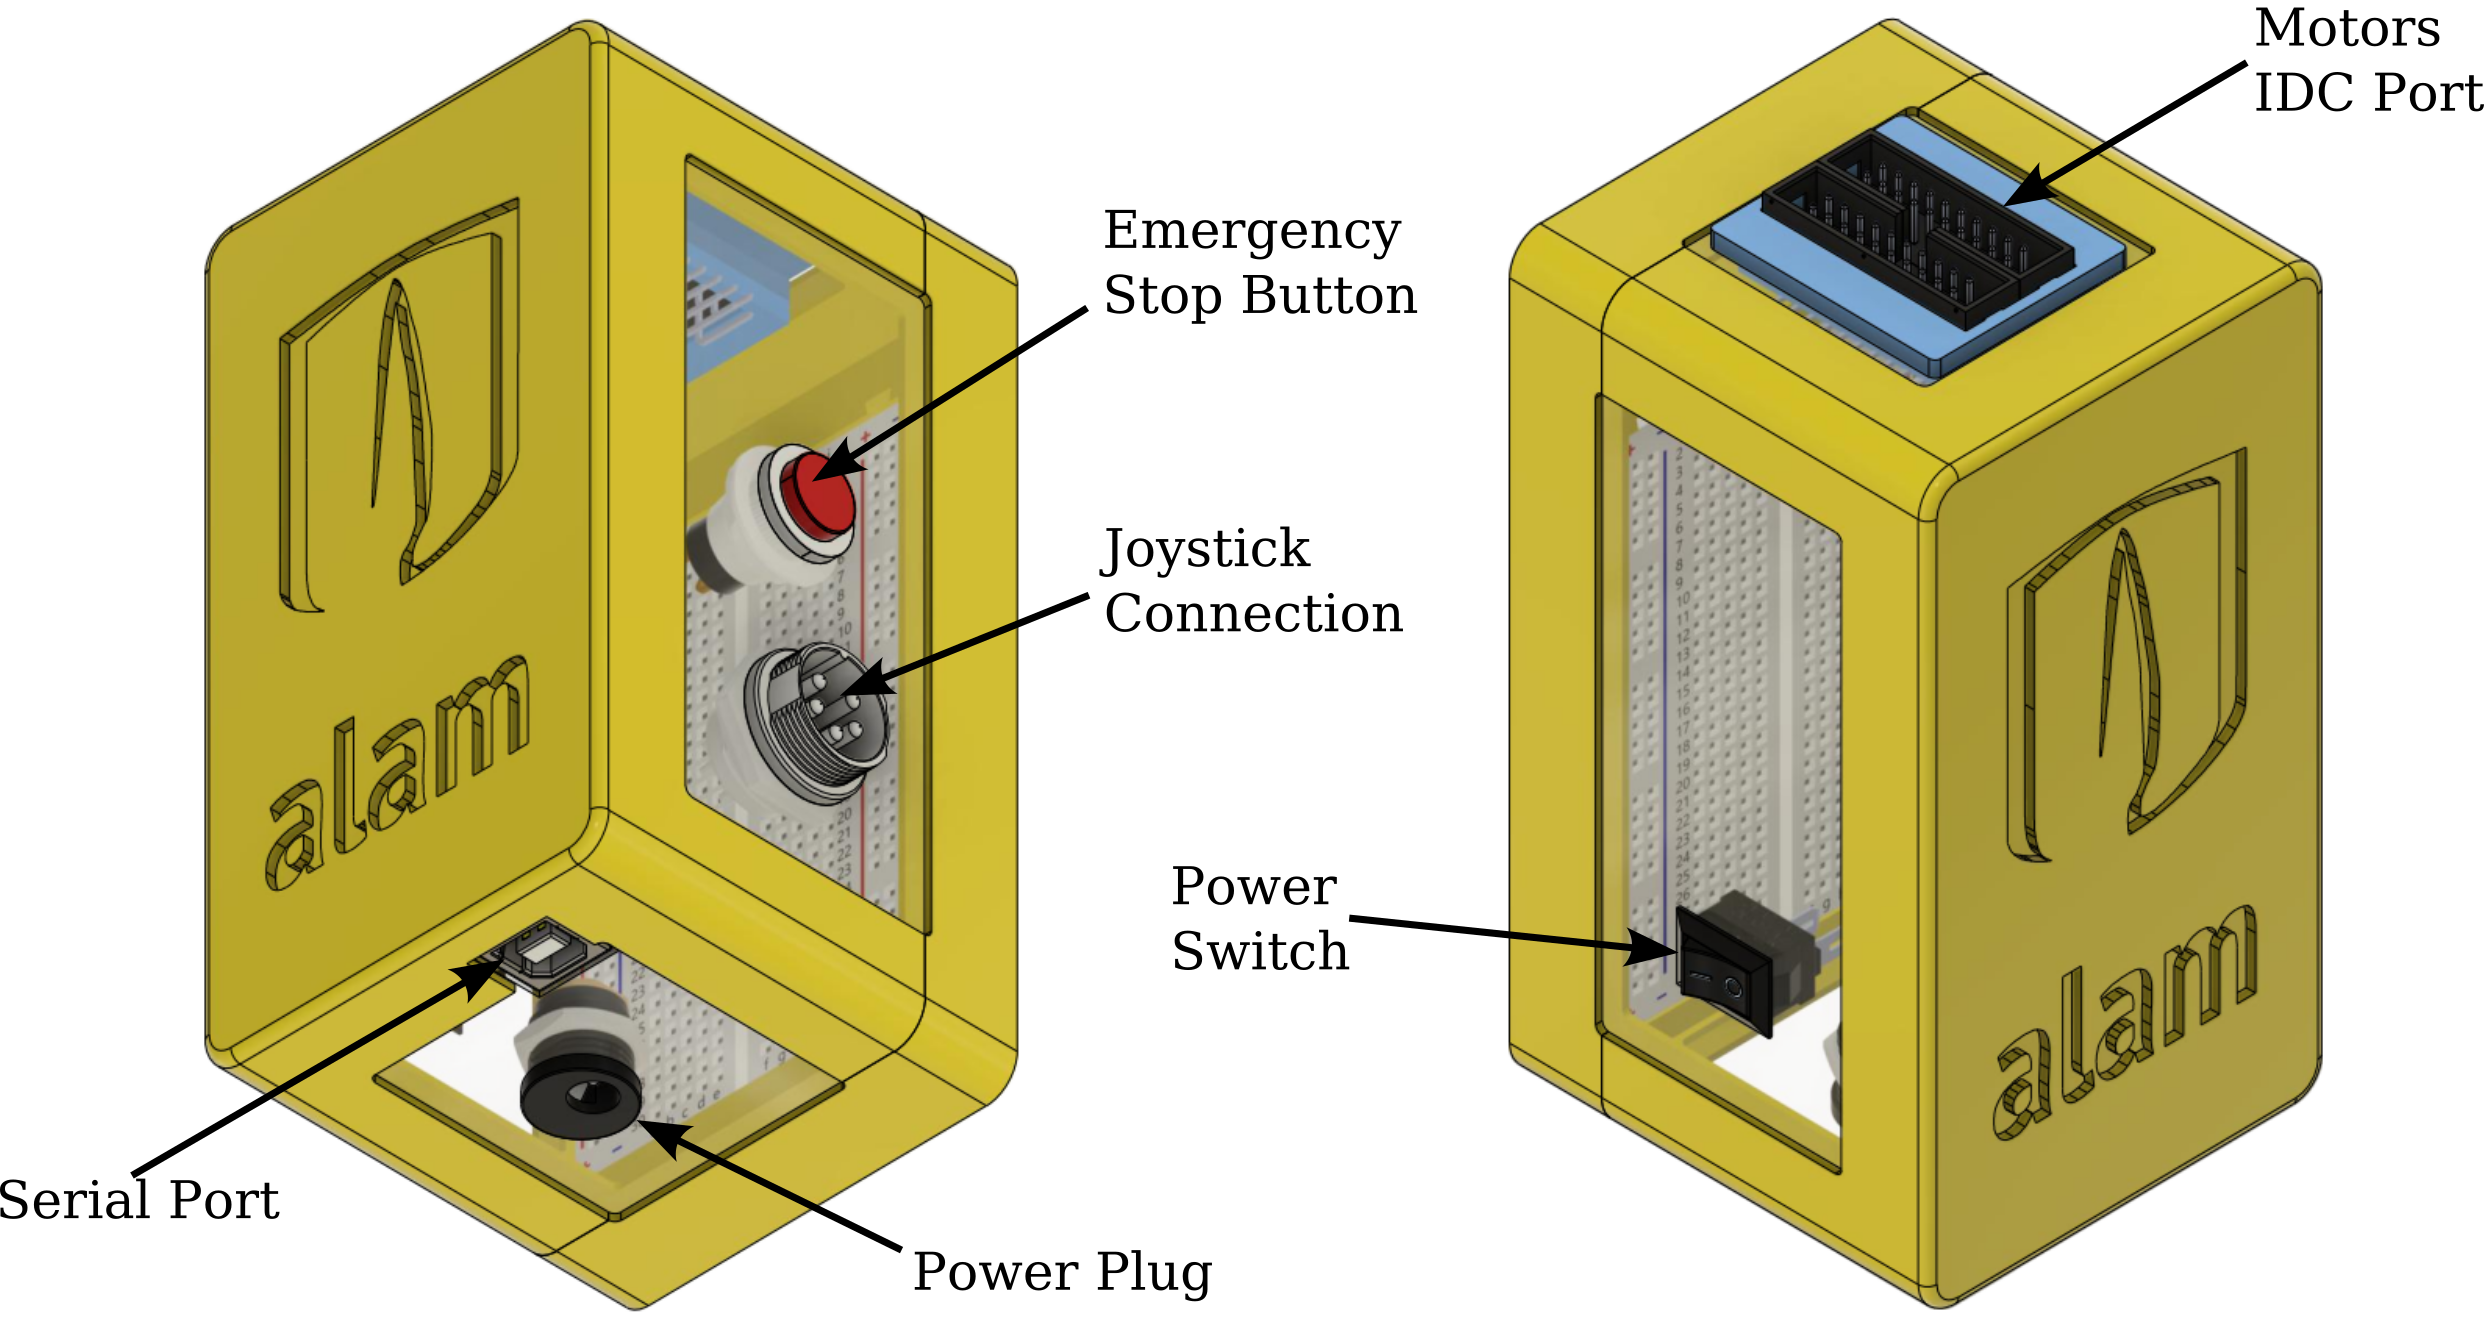
\includegraphics[width=0.85\textwidth]{electronics-ports}
    \caption{Ports and connections}
    \label{fig:electronics-ports}
\end{figure}

\subsection{Circuit Schematic}
The schematic of the circuit connections is illustrated in Figure \ref{fig:main-circuit}. As shown in Figure \ref{fig:motor-circuit}, each actuator motor requires six connections. The pins \texttt{M1} and \texttt{M2} supply power to the motors, while \texttt{VCC} and \texttt{GND} provide power to the magnetic encoder. The pins \texttt{A} and \texttt{B} are used for quadrature output. To accurately count the encoder pulses in both directions, one pin must be connected to an interrupt pin and the other to a digital pin. Motor polarity and speed are managed using a \texttt{DRV8833} motor driver, which requires two \texttt{PWM} connections per motor. Given the need for a cost-effective MCU with sufficient pins to connect six motors, the \texttt{Arduino MEGA 2650} was selected for this project.

\begin{figure}
    \centering
    \includesvg[width=\textwidth]{main-connection2}
    \caption{Main circuit schematic}
    \label{fig:main-circuit}
\end{figure}

\begin{figure}
    \centering
    \includesvg[width=\textwidth]{motor-connection2}
    \caption{Motor circuit schematic}
    \label{fig:motor-circuit}
\end{figure}
